%\documentclass{sig-alternate}
\documentclass[conference]{IEEEtran}

\usepackage{graphicx}
\usepackage{pifont}
\usepackage{url}
\usepackage{code}
\usepackage{amsmath}
\usepackage{caption}
\usepackage{algorithm}
\usepackage{multicol}
%\usepackage{fontspec}



\usepackage{algpseudocode}
\usepackage{listings}
\usepackage{xcolor}

\lstdefinestyle{BashInputStyle}{
  language=java,
  basicstyle=\small\sffamily,
  numbers=left,
  numberstyle=\tiny,
  numbersep=3pt,
  frame=tb,
  linewidth=0.9\linewidth,
  xleftmargin=0.1\linewidth
}


\definecolor{dkgreen}{rgb}{0,0.6,0}
\definecolor{gray}{rgb}{0.5,0.5,0.5}
\definecolor{mauve}{rgb}{0.58,0,0.82}

\lstset{frame=tb,
  language=Java,
  aboveskip=3mm,
  belowskip=3mm,
  showstringspaces=false,
  columns=flexible,
  basicstyle={\small\ttfamily},
  numbers=none,
  numberstyle=\tiny\color{gray},
  keywordstyle=\color{blue},
  commentstyle=\color{dkgreen},
  stringstyle=\color{mauve},
  breaklines=true,
  breakatwhitespace=true,
  tabsize=3
}


\newcommand{\comment}[1]{}

% correct bad hyphenation here
\hyphenation{op-tical net-works semi-conduc-tor}

\def\mytool{hddRASS}
\def\mytitle{Hierarchical Delta Debugging for resource adaptive software system}


\begin{document}
%
% paper title
% Titles are generally capitalized except for words such as a, an, and, as,
% at, but, by, for, in, nor, of, on, or, the, to and up, which are usually
% not capitalized unless they are the first or last word of the title.
% Linebreaks \\ can be used within to get better formatting as desired.
% Do not put math or special symbols in the title.
\title{\mytool : \mytitle}


% author names and affiliations
% use a multiple column layout for up to three different
% affiliations
\author{
\IEEEauthorblockN{Arpit Christi}
\IEEEauthorblockA{School of EECS\\
Oregon State University\\
Corvallis, Oregon, USA\\
christia@oregonstate.edu}
\and
\IEEEauthorblockN{Alex Groce}
\IEEEauthorblockA{School of EECS\\
Oregon State University\\
Corvallis, Oregon, USA\\
agroce@gmail.com}
\and
\IEEEauthorblockN{Rahul Gopinath}
\IEEEauthorblockA{School of EECS\\
Oregon State University\\
Corvallis, Oregon, USA\\
gopinatr@oregonstate.edu}
}

% conference papers do not typically use \thanks and this command
% is locked out in conference mode. If really needed, such as for
% the acknowledgment of grants, issue a \IEEEoverridecommandlockouts
% after \documentclass

% for over three affiliations, or if they all won't fit within the width
% of the page, use this alternative format:
% 
%\author{\IEEEauthorblockN{Michael Shell\IEEEauthorrefmark{1},
%Homer Simpson\IEEEauthorrefmark{2},
%James Kirk\IEEEauthorrefmark{3}, 
%Montgomery Scott\IEEEauthorrefmark{3} and
%Eldon Tyrell\IEEEauthorrefmark{4}}
%\IEEEauthorblockA{\IEEEauthorrefmark{1}School of Electrical and Computer Engineering\\
%Georgia Institute of Technology,
%Atlanta, Georgia 30332--0250\\ Email: see http://www.michaelshell.org/contact.html}
%\IEEEauthorblockA{\IEEEauthorrefmark{2}Twentieth Century Fox, Springfield, USA\\
%Email: homer@thesimpsons.com}
%\IEEEauthorblockA{\IEEEauthorrefmark{3}Starfleet Academy, San Francisco, California 96678-2391\\
%Telephone: (800) 555--1212, Fax: (888) 555--1212}
%\IEEEauthorblockA{\IEEEauthorrefmark{4}Tyrell Inc., 123 Replicant Street, Los Angeles, California 90210--4321}}




% use for special paper notices
%\IEEEspecialpapernotice{(Invited Paper)}




% make the title area
\maketitle


\begin{abstract}

	Building software systems that adapt to changing resource environments is challenging: developers cannot anticipate all future situations that a software system may face, and even if they could, the effort required to handle such situations would often be too onerous for practical purposes. We propose a novel approach to allow a system to generate resource usage adaptations: use delta-debugging to generate versions of software systems that are 1-minimal with respect to satisfying various (labeled) subsets of a system's test suite. Many such variations will, while retaining core system functionality, use fewer resources. We describe an efficient tool for computing such variants and show how it reduces with respect to randomly selected subsets of Java class test suites, and propose an infrastructure in which this approach leads to a method for resource adaptation in the field. Using the NetBeans IDE, we demonstrate that even without additional infrastructure or heuristics, our approach is capable of quickly and cleanly removing a program's undo functionality, significantly reducing its resource usage, with no more effort than simply labeling three test cases as undo-related.
\end{abstract}

\section{Introduction}

Modern day software systems are very complex consisting of various resources like libraries, models, operating systems, databases, memory systems, processors drivers, browsers, services, data structures etc. While developing such complex software systems, certain implicit or explicit assumptions are made for the resources that either software is going to use or the software is going to be operated under. For example, a mobile application using location assumes that some sort of location provider services is available via network or GPS or through some other mechanism. Advances in underlying technology, sometimes continuous or sometimes drastic forces software developers to adapt/evolve their software to these underlying changes. Users of such systems have to go through updates in software or sometimes buying new technology to continue to use certain software. A change in a library used by the software sometimes forces developers to refactor or rewrite part of their software which can lead to multiple cycles of development and testing before the application can be fully adapted to the library changes, a costly, time consuming and error prone process.  

Having a mechanism to design and implement resource adaptive real world software system that can adapt to changing environment or changing resources can solve the problem. A lot of work has been lately devoted to building self adaptive software system.s. In their survey of engineering approaches for self adaptive software systems Crupitzer et al discussed different approaches to build self adaptive software systems \cite{selfAdaptation2}.     

In order to design and implement resource adaptive software system for mission critical industry strength software system, DARPA launched Building Resource Adaptive Software System project, BRASS, that employs a new clean slate approach that aims to capture the relationship between computations and the resources they use and provide transformations that enable applications to adapt to resource changes without the need for extensive programmer involvement \cite{darpa1}. 

As per vision of BRASS, When applications adapt to resources that adaptations are manifested as (1) Restricted functionality (2) Altered functionality and (3) Enhanced functionality. We observed and worked with a team of developers trying to build resource adaptive software system and realized that developers design and implement applications react to these adaptations by reduction or replacements mostly. In reduction, the system adapt to depleted or changing resource need by reducing the application functionality, by not respecting less significant or low priority invariants while still observing significant and high priority invariants. Basically, the application continues to provide some(mostly important) functionality while avoiding exercising some features. In replacement, application adapt similarly but by changing some functionality by equivalent functionality such that resource under stress is less utilized.  

Resource adaptive software systems (RASS) are designed and implemented mostly for mission critical software systems and normally accompanied by a good test suite that captures the specifications of the system well and does a thorough job in verifying these specifications. There is a normal consensus among the developer that whenever system adapts and reduction is the chosen adaptations, it may not be able to observe all the invariants all the time. Sacrificability of specifications can be captured using a test suite by extending the test suite at test case level, at an invariant level or using some other complex combinations for reduction based adaptations. It can be as simple not exercising all the test case that exercise a single feature or turning off some asserts that verify state change of function call.  Now if we have a systematic program reducer, we can reduce the program, component, class or method automatically to adapt to resource need based on the extended test suite. 

This paper proposes a methodology to automatically create a reduced variant(s) of the program based on sacrificability of specification captured by extended test suite.  Developers can manually annotate test cases or assertions one by one or can employ some automatic mechanism to achieve these annotations. It achieves accurate program reduction by using \mytool, a new tool that we are proposing,  that combines HDD with statement deletion mutation, to automatically create this reduced variant of the program. The basic adaptation workflow is as follows. (1) Developer annotate the test suite of the program. (2) Program is deployed with its annotated test suite and newly proposed tool, \mytool\ . (3) When resource adaptation is triggered, using annotated test suite and current program, \mytool\ finds out minimal working version of the program.

This paper proposes and implements a tool, \mytool\ that takes as its input a program and an extended test suite and via reduction find out the minimal program such that all tests at certain level in extended test suite will continue to pass. The methodology and tool proposed as part of our work can be considered a step in the right direction in ensuring system reliability of mission critical system that works in an environment where resource availability is unpredictable. %Previously reduction tools have been proposed but they are mostly proposed to keep the failure or bug isolation than to produce a useful version of the program, they do not necessarily fit into or optimized for the proposed adaptation work flow. Delta-Debugging(DD) or Heirarchical Delta Debugging(HDD) are also well known reduction algorithms \cite{ddOriginal,hddOriginal}. Tools like chipperJ \cite{chipperJ} and picireny \cite{pricieley} were previous implementations of HDD that apart from reducing test input, can reduce java programs also. We will discuss advantages of our tool against these tools in related work section, most important distinction being its ability to optimally fit into adaptation workflow.  The \mytool,  as a stand alone tool,can reduce any java program given a JUnit test suite. The tool is also flexible such that by implementing an interface it can be extended to accommodate any arbitrary test suite. We have successfully used it to reduce real world android application and multiple open source java projects. Though tool was originally designed to build reduced component to aid building resource adaptive software system, it is a general purpose reduction tool that can reduce java programs using test suite. %  

Our contribution is as follows: 
\begin{enumerate}
\item We proposes a workflow that employs extended test suite, a newly developed reduction tool and existing program to automatically build adaptive program.
\item We propose test case labeling/annotations as a way to capture sacrificability of specifications.
\item We implement a stand alone reduction tool \mytool\, to build adapted version of the program using extended test suite. \footnote{our tools is available at https://github.com/amchristi/hddRASS}.
\item To demonstrate the usefulness of our methodology, we \emph{automatically} build an adaptive NetBeans IDE by just labeling 3 test cases that can reduce memory consumption significantly by sacrificing redo-undo functionality.
\item We demonstrate that \mytool\ is highly applicable, accurate and works out of the box for most of the java program setups
\item Empirical evaluation of reductions achieved using extended test suite using real world large open source programs.
\end{enumerate}      


Remaining paper is organized as follows. In section 2 we provide we describe some of the related work and how our tool differs from existing tools. In section 3 we provide background of component based approach of building adaptive software system in practice and motivation behind our approach. In section 4, we describe methodology to achieve pre-computed and run time adaptations using our tool and test case annotations. In section 5 we provide description of the tool, the theoretical aspects, practical considerations, architecture, algorithm, implementation, usage and challenges. In section 6 we evaluate the method by building adaptive NetBeans IDE that consumes less memory. Section 7 evaluates our tool and studies the reductions produced by our tool. Section 8 contains future work and conclusion.  


\section{Related work}

The current status of work and challenges for self adaptive systems are well summarized in the work of Salehie et. al. \cite{selfAdaptation1}. They also summarize some work done in practice by some of the organizations. Kruptizer et. al. \cite{selfAdaptation2} discusses different engineering approaches used in building adaptive software systems. The approaches they discuss include but not limited to model-based, architecture-based, reflective, programming paradigms, control theory, service oriented, agent based, formal modeling and verification based, machine learning based and others \cite{selfAdaptation2}. Tactical Situational Awareness (TSA) system that we worked with falls somewhere between Model based approach \cite{modelBasedAdaptation} and Architecture based approach \cite{architectureBasedAdaptation} to build self adaptive software systems.  


Alex or Arpit - if space permits, add something mentioning slicing.

Delta-debugging (DD/dd for short) is an algorithm for reducing the size of failing test cases or test inputs \cite{ddOriginal}. Hierarchical Delta Debugging \cite{hddOriginal} or HDD/hdd was proposed to efficiently reduce test inputs that are hierarchical in nature, for example, html inputs, xml inputs and programs. When programs were reduced earlier using HDD, the reduction criterion were simpler like keeping the crash. Many HDD implementations have been proposed previously, including a very recent one priceley \cite{hddOriginal,chipperJ,pricieley}. Early HDD algorithm paper has reducer for C program \cite{hddOriginal}. CReduce was proposed to reduce C Programs generated to find compiler bugs in C program \cite{cReduce}. First of all our tool differs from those tools in its intended usage. Almost all other tools were designed to reduce test inputs to find the smallest failing test input. Our tool try to reduce program with intention to find a reduced but useful version of the program that does not respect certain specifications as specified in test suite. Most of the previous program reducers find minimal configuration using AST (like we do), most of them does not rely on statement deletion as their primary reduction step \cite{hddOriginal,hddOriginal} 

Also, all other tools, because they do not need to respect any property that does not contain failure, normally produce outputs that are significantly smaller then original output. Most of the papers boast their reduction factors and compare with other approaches using reduction factors \cite{hddOriginal,chipperJ,pricieley}. In order to quickly generate those reduced input, they tend to have bigger chops earlier when they reduce. In our case, a program and its reduced version will have few dissimilarity as the reduced program is expected to be a useful artifact itself, our algorithm (1) starts with the smallest unit possible (sentence, in our case) and (2) Start with leaf nodes and build upwards.  

Authors of the most recent tool picinery  \cite{pricieley}, lamented the fact that no newer HDD tools came out for long years and older tools use very outdated technology. Authors also acknowledge the fact that HDD tools are not used in practice. They proposed a new tool, picinery, where they use homogeneous technology component (every underlying component of their tool uses python) and used modern libraries like ECFG ( Extended CFG) instead of CFG(Context Free Grammer). Authors definitely modernize HDD, but did not mention how their tool will encourage widespread industry usage. 

%chipperJ reduces java programs for automated bug isolation and was successfully applied to reduce complex java programs for bug isolation \cite{chipperJ}. chipperJ rely on very naive symptom like null pointer exception or looking for particular string in the output and cannot be used for general purpose standalone tool with modern day software without significant changes.%

Most HDD (and DD) implementation assumes ability to provide test results into HDD implementation in the format that the tool wants. That means a practitioner will have to make sure that they write some sort of test script and plug in the results in the format the tool expects. picinery has \texttt{test \"put your test script here\"} option in command and chipperJ architecture figure has a test script block supplying results to chipperJ.  Before any HDD reductions will start, a pre processing step is expected and mostly performed when HDD tools are run for research purpose. 

Rahul writes about statement deletion mutatation. 
Rahul writes about unchecked coverage.
 
%With modern day software system, there is an ecosystem of programming and testing technology. Most of the open source and even industry Java projects have their tests written in JUnit. Same is true with other programming languages like C\#, javascript etc. HDD tools fail to leverage this fact leaving some of the work as pre-processing for developers. As we will discuss later, hddRASS is a complete standalone tool that requires no pre-processing if Java/Android program is used with Junit \cite{junitHome} test suite. Also, as we will discuss in tool section, our tool is easily extendable to other test framework in the ecosystem.
%
%Mutation \cite{mutation} was technique to inject fault in the program to measure effectiveness of the test suite. SDL \cite{sdlMutation} is statement deletion mutation. HDD based program reductions are essentially applying SDL mutation at each step of reduction. They just apply it in a very systematic way with the end goal of keeping the fault and building on the last useful mutant generated until a local minimal mutant is found, in our case, end goal is keeping program correct with respect to test suite.%    
 

    

   


\section{Background and Motivation}

We are working with a group of developers trying to build real world resource adaptive software system, the system that is being built is known as Tactical Situational Awareness System also known as SA - Situational Awareness. To demonstrate the design and implementation of resource adaptive software system, we will use location provider of SA as an example, that sends location of people or object carrying the device to some server. Location provider in case of SA consists of location, image and sometimes streaming video of the location, more complex then normal location providers where location itself is enough. Also location provider of SA can be used in extreme locations like in remote battlefield, forests or under sea where resource availability is drastically different then the environment in which SA and location provider is implemented. Devices that SA is deployed on can have very varying hardware and depending upon the the environment system is forced to use network or GPS for location. The quantity and quality of resources are not known in advance and vary drastically.

Specification of such systems are well documented and verified sometimes using a good test suite. Though, to adapt to extreme resource need some of these specifications are relaxed or compromised at run time in practice to let system function in deteriorated way. For instance, if system sends latitude, longitude, altitude and image as part of location provider, in case of low network bandwidth, system choose not to send the image, at least you know where the person or vehicle carrying the system is. Another example of adaptation can be turning off logging functionality if disk space is really low, helpful in case your disk is inside a satellite where immediate maintenance is not possible.

Component based approach to adaptive software development assumes a software system to be built of loosely connected components that are replaceable, sometimes even at run time \cite{architectureBasedAdaptation}. So, when resources are sparse or unavailable, making a particular software component unusable in its current state, system tries to swap it with a replaceable component in such a way that component and hence the system will continue to run in the changing and most often deteriorated resource environment, giving system a better chance to survive, making system more reliable.

As per objective and system evaluation of BRASS, adaptation for resources by a system can manifest itself in various ways \cite{darpa1}, the most basic being \begin{itemize}
\item Restricted functionality - Resource based adaptations will not observe certain system specifications, making system limited in its functionality. Just like low network bandwidth will trigger adaptations that will not send images.
\item Altered functionality - Resource based adaptations will observer some specifications in altered way then originally intended. In previous example, images will be send periodically while location will be sent at normal rate.
\item enhanced functionality - Resource based adaptations will meet all the specifications and may now meet some new specifications that the system was not originally implemented for. These kind of adaptations are not going to part of the discussion of this paper.  
\end{itemize}

%In this section we motivate the need of a tool that combined with test suite  can automatically produce reduced version of the components used as building block of adaptive software system. We also argue that though the tool is designed to aid building/mutating components of resource adaptive software systems, it is general tool that can be used to reduce any java program with respect to a test suite. %

As part of the BRASS effort to build industry strength resource adaptive software system that can last 100 years \cite{darpa2}, we closely work with a team of developers attempting to do so. We observed how they try build the components with possible adaptations in mind. Though authors acknowledge the lack of empirical analysis partly because unavailability of subjects as rarely systems are implemented as resource adaptive software systems, we observe that developers tend to employ two different natural strategies.

\begin{enumerate}
\item Reduction - Developers build reduced version of original components that does not observe certain less critical specifications.
\item Replacement - Developers build components that are altered from original components, new components use different libraries, data structures, hardware, resources etc.  
\end{enumerate}

Reduction makes most sense when it is possible to shield the component and in turn system by relaxing some of its specifications either by turning off some features or by not executing certain part of the code such that resource under stress will be less utilized or not utilized at all. Replacement makes most sense when it is possible to come up with completely different components using completely different libraries, hardware, data structures etc such that it will alter the resource usage also making application weather the resource degradation. Reduction associate with Restricted functionality and Replacement with altered functionality objectives mentioned by BRASS objectives as mentioned in background section. For remaining of the discussion we are only going to consider reduction strategy.   

Currently both the strategies are executed manually. A developer has to carefully observe the component, observe its resource need, consider the specifications, wrap her head around component interactions in order to come up with correct reductions. Also the reduced components have to be identified, associated with and verified against its resource consumption. They have to be verified against the \emph{new or reduced set of specifications} they are going to observe. All these steps are manual, error prone and tedious. It also triggers few cycles of development and testing. 

Is it possible to automate this process? The methodology, test suite extension and \mytool\ discussed in further sections are motivated with the intentions to (1) help developers to quickly and automatically build reduced components that can fit into resource adaptive software when reduction is the chosen adaptation. (2) If runtime adaptations are triggered and already built component is not found, system can build a new reduced component at run time.  


%\input{formal}
    
\section{Methodology}

This section discusses the methodology to automatically build reduced components for resource adaptive software using extended test suite and \mytool\. As we discussed previously either adaptations are pre computed by developers or it can trigger at run time if a pre computed adaptations are not available.
 %For java programs, pre computed adaptations can be computed using source code or bytecode but run time adaptations can be computed only using bytecode as source code is not available at run time.%
Developers based on the context knowledge of system and its environment, chooses pre computed adaptations or run time adaptations. Providing multiple reduced components for each of the system component can make system bloat in its size and may create performance issues while system is still functioning in normal environment in some cases. Run time adaptations will pause system until adaptations are completed and then swap it with original component. Pre computed adaptations are useful if adaptations are needed frequently and providing pre computed adaptations does not create serious performance issue. Run time adaptations are useful if adaptations are needed rarely and can be triggered quickly or pre computed adaptations are not available.   

\subsection{Labeling test cases}

Extending test cases is nothing but to prioritize test cases as per its importance and embed this information as part of test case itself. For Junit test cases, this is achieved by providing annotation for each of the test case, we call this labeling of test cases. Test cases are labeled from 0 to n, test cases with label 0 being the most important test cases. If any of these tests fail that means system is not usable. Test cases with label n are the least important and the specifications observed by these test cases can be sacrificed without affecting system seriously. Test cases with label closer to 0 are more important then test cases with label closer to n. This process divides test cases in n different level. Test case labeling can be manual or automatic. In manual labeling, developer will go through the tedious task of going through each test case pertaining to a component and label them. Work on automatic labeling is under progress hence for rest of the paper, we assume manual labeling. Also, labeling cane be applied at coarser or finer levels giving us tighter or loose reductions. For Junit test cases, labeling can be applied at test class level or at each assertion level in turn making life of developer easy or difficult. 


\subsection{Workflow for pre computed adaptations}
\begin{enumerate}
\item Developer extend the test suite by labeling each test cases or each assertions. 
\item For each of the level, starting from level n we do the following.
\item If current level is x, remove all the test cases whose label is k, k  x.
\item Provide remaining test suite and program or component as input to \mytool\. abcd
\item The tool outputs minimal program/component for level x.   
\end{enumerate} 

\subsection{Workflow for run time adaptations}

\begin{enumerate}
\item Developer extend the test suite by labeling each test cases or each assertions.
\item Run time adaptations are triggered and we assume reduction is chosen adaptation.
\item Start with level n and do the following
\item remove all tests labeled as k where k is greater then n. 
\item Provide remaining test suite and program as input ot \mytool\
\item \mytool\ outputs minimal program. check it against resource contraint.
\item If resource constraint is not violatedm keep the reduced program.
\item If it is violated, continue by reducing by one level. 
\item If level 0 is reached, stop and output that system cannot be used under given resource constraint.
\end{enumerate}

\subsection{Choosing only subset of tests}
For object oriented components, components are reduced by reducing all the classes and classes are reduced by reducing all the methods. When a class is being reduced, as we will discuss in Tool section, after each unit reduction step, system needs to be compiled and tests need to be executed. Running all the tests of a component when we just reduce a single class can be prohibitively time consuming as this step has to be repeated large number of times. To speed up the process, we only choose a subset of tests from all the tests such that only most relevant tests for the class will be selected. For instance, for Apache commons validator project, changing specification of URLValidator does not affect behavior of CreditCardValidator or CalendarValidator and hence all or some tests testing CreditCardValidator or CalendarValidator need not to run when reducing URLValidator. We find similar situation while working with TSA system also. To accommodate the situation and to allow quick convergence, \mytool allows its user to specify set of tests out of whole test suite at test class level. hddRASS will only run those tests during the reduction process, saving significant amount of time and resources. Selecting tests is not possible when run time adaptations are triggered on a deployed system.In their cloud refactoring work, kwon and Tilervich proposed a way to choose \emph{corresponding methods/classes}  by a process that they call profile based recommendations that rely on static analysis and dynamic traces. Based on that, they define two terms CC - Class connection and CR - Class Relation and provided recommendations based on that. Value of CC and CR can be from 1 to 0, with 1 means most tight connection or strong relation and value 0 means no connection or no relation. We also do static and dynamic analysis of our program and tests and recommend tests for a class based on Kwon's method but employing much simpler formula. For simplicity, we select a test case only if CC and CR both are 1. Allowing CC and CR thresholds to be less then 1 will select more tests as \emph{corresponding tests}. This will increase the time required to converge the reduced class and decreases the amount of code reduced as the class is tested against more specifications. CC and CR value being 1, if simply put in words means, test case directly calls a method of the class in code and that method was indeed executed during the execution of the tests. CC and CR values should be left as configurable parameters that can be adjusted based on the context.      


\section{Tool}
\label{sec:experiments}

In this section, we discuss intuition behind combining HDD with statement deletion mutation to develop \mytool\  such that it fits into adaptation workflow, modified HDD algorithm, architecture, implementation and usage of the tool in detail.       

\subsection{coverage and dead code removal}
It is important to note that if the program parts that can be reduced only contains non covered entities, just computing coverage and removing non covered entities will do the job. But even if entities are covered, but does not contribute to the correctness of program as defined by test suite, they qualify as reduction candidates. Though \mytool\ can be optimized by allowing non covered entities to be reduced first, something we are planning to do in future. To provide an example, consider following code that was removed as part of our reduction from URLValidator class.

\begin{lstlisting}[caption={URLValidator reduced code}]
if (!isValidAuthority(authority)) {
	return false;
}
\end{lstlisting}

The code was reduced when we relaxed specifications by randomly turning off 2 tests. The code was reduced though it was \emph{covered 42018 times during execution}. 

%At any point in the reduction step, we are essentially creating a statement deletion mutant or a combination of multiple statement  though with the purpose of creating a useful version of the program instead of injecting a fault. We start the process from leaf nodes, if we find a useful SDL mutant, we keep it and use it for rest of the process until local minimal is reached.%  


\subsection{1-minimal program}
\label{sec:opensource}

Original delta debugging work defines different notions of minimality for reduction in detail \cite{ddOriginal}. For our further discussion, we define 1-minimal program or 1-minimal mutant as follows. It is important to note that this is local minimal as DD or HDD are greedy and our algorithm is also greedy \cite{ddOriginal, hddOriginal}. Given a program P and a  test suite T, we define 1-minimal (local) program P' of P is the reduced version of P such that all tests continue to pass and the program cannot be reduced further. For component level adaptations, the idea of 1-minimality is applied at component level. The intention of hddRASS is to output the 1-minimal program for a given program given a test suite such that all tests continue to pass. 

\subsection{Statement Deletion mutation - SDL}
\label{sec:sdl}

If resource adaptation is triggered because of resource constraint violation and if a reduced program/component is generated, as the reduced program is still a useful artifact that will continue to function as it is mostly, we hypothesize that small local changes are applied to the program. The newly created program is a perturbation of the original program and mutation captures perturbations well. In traditional mutation testing, purpose of the mutant is to act as an artificial bug while in our case mutant is a useful perturbed version of original program. Rahul write this statement: Statement Deletion mutation operator was proposed by xyz and during empirical analysis conducted by abc it was found to be very effective and it subsumed other mutation operator significantly. When HDD is traditionally applied on programs, it relies on tree structure of the program like AST, CFG or ECFG etc. For example, picireny relied on ECFG of programs. Its reduction run even deeper then program statements, it even reduces expressions. Our approach does not go beyond SDL because (1) SDL operator was found to be subsuming other mutation operator that are used in expressions (2) As reduced program still needs to be working as mostly correct program, we expect simple removals. (3) Minimally reducing expressions, conditions etc further may be very time consuming and hence runtime adaptations may not converge quickly.

   


\subsection{Intuitive modification to HDD for RASS}
\label{sec:intutive}
Now we describe modifications that we propose to original algorithm and intuition behind the proposals. Later during evaluation we find some evidence for the intuition. We need to put on our \emph{Resource Adaptive Software System developer} hat on to understand this modifications. As the reduced adaptive program is a useful artifact that will be used in place of the original software, we hypothesize that (a) it may not be drastically different then the original program. (b) Any reduction that does not compile is useless.

(1)  Reduction may incur many small local changes to software based on the relaxed specifications. As original HDD setups were designed to quickly converge to reduced input that is significantly \emph{smaller} then original input, they tend to make bigger chops earlier in the process. As changes to RASS are going to be local and smaller, we propose modification to original algorithm. Our algorithm always start with leaf nodes at highest depth level and it chops smallest possible unit at the beginning (statements for our tool). 

(2) Consider any two statement s1 and s2 existing at the same level in AST in the order s1,s2. Our algorithm always delete s2 before s1. Our deletions are always from right to left at same level in AST. (a) This prevents some posibilities of non compilable code and hence costly reverts, use will always be deleted before def. (b) Later read/write will be deleted before earlier read/write. Will this have better chance to keep program correct, for Alex to answer? Reverts will be needed only if any test in test suite failed.    

(3) Consider any two statements s1 and s2 existing at different level in AST such that s1 is at higher level. As our algorithm starts from leaf node and moves upward, s2 will be deleted before s1 ensuring that if def and use are at different levels, use will be deleted before def, again reducing possibility of non compilable code.  



\subsection{Algorithm}
The basic algorithm is described below. It still follows all the standard steps of HDD, though it is modified to fit into adaptation workflow better by taking into consideration modification mentioned in previous section. 

\begin{algorithm}
\caption{Hierarchical Delta Debugging}
\hrulefill
\begin{algorithmic}[1]
\Procedure{hdd}{$inputTree$}
    \State $level\gets\textsc{HigestDepthLevel}(inputTree)$
    \State $nodes\gets\textsc{TagNodes}(inputTree,level)$ 
    \While{nodes are not empty}
	\State $minConfig\gets\textsc{ddmin}(inputTree)$
	\State $\textsc{prune}(inputTree,level,minConfig)$
	\State $level = level - 1$
	\State $nodes\gets\textsc{TagNodes}(inputTree,level)$ 	
	\EndWhile

    \State \textbf{return} $level$ 
\EndProcedure
\end{algorithmic}
\hrulefill
\end{algorithm}
\label{sec:algorithm}


\subsection{Architecture and implementation}
\label{sec:architecture}
\begin{figure}
  \centering
  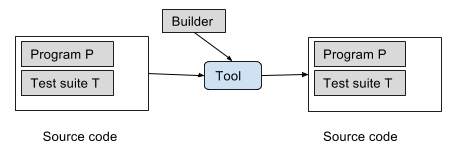
\includegraphics[width=1.0 \columnwidth]{basic_tool_architecture.png}
  \caption{Overview of the tool}
  \captionsetup{justification=centering}
  \label{fig:fig1}
\end{figure}



The basic architecture of the tool from a user's perspective is shown in figure ~\ref{fig:fig1}. For Java-JUnit combo, user just needs to provide the source code that consists of the program and labeled tests for java projects.The only extra information needed is a build command - ant, gradle or maven command for modern day java projects. No separate mechanism is needed to feed DD with pass-fail result by setting up a tester, running it and collecting the results. 

Figure ~\ref{fig:figDetailedToolArch} describes the detailed architecture of the tool. Components in oval gray are input/output, original program P, Test suite T, and builder constitute input and Program P$'$ is output. Components in white rectangle constitute part of the tool. Architecture follows standard HDD/DD procedure of reduction while taking into account the changes proposed in intuitive modification subsection. Program is passed to AST Parser \cite{javaparser}, we used JavaPaser for this. We implemented our own HDD to reflect changes mentioned in intuitive modification subsection. Similarly, we have our own implementation of DD for the reasons mentioned in intuitive modification subsection. Apart from implementation/algorithmic changes that we proposed, the major architectural change consists of how test results are being fed to dd. Tools like picireny and chipperJ require some sort of test script and pre-processing for developers, while testing is built in as part of our tool. 			

\begin{figure*}
  \centering
  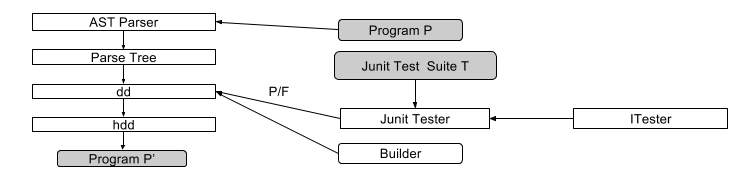
\includegraphics[width=1.8 \columnwidth]{detailed_tool_architecture.png}
  \caption{Architecture of the tool}
  \captionsetup{justification=centering}
  \label{fig:figDetailedToolArch}
\end{figure*}


\subsection{Usage}
Tool takes as its input, a program (or a component if only component needs to be reduced), a test suite or a tester, a build system and produces a \emph{minimally reduced program} such that all test cases continue to pass.  Though right now it works as a stand alone tool with JUnit tests only, the tool is very extendable and flexible to accommodate any other testing technologies. Just like JUnitTester in the ~\ref{fig:figDetailedToolArch}, providing an extra implementation, NUnitTester, will make the tool capable of working with any java projects consisting of NUnit test suite out of the box. Tool can be easily extended to work with other arbitrary tester by implementing a simple interface that consists of only one method. We were able to extend it for TSA system under consideration that has a customized tester written in python by implementing the interface using less then 70 lines of java code. Tool is made available as command line tool with many flexible options giving developers very fine control over how it can be used. Tool can be used at method level, class level, program level or component level giving its user finer control over reduction. 








\subsection{Challenges}
The challenges that we faced are very similar to other reduction tools. 

\begin{enumerate}
\item Non complilable code - Most of other tools discussed in this paper, just revert the code if code is not compilable at any step of reduction. This issue is not present in our implementation by design, we attempt to produce code that compiles only. Though we still compile at the end of each reduction step (just like other tools) in order to make sure that our reductions are at any point of time are compilable indeed. Because of our proactive approach, we are able to avoid reverting, one of the most time consuming step, reverting mostly require writing back java files. 
\item Infinite loops - This problem is just not avoidable as reduction can delete loop control statements. We employ very crude strategy of providing some threshold and giving up if the threshold is hit and returning Fail as result of tests. 
\item Local minimum - As mentioned earlier, nature of ddmin or hdd just produces local minimum and as our tool is built on hdd, our tool also produces local minimum program.
\end{enumerate}






\section{Evaluation methodology}

acbd

\begin{table*}
\begin{center}
\begin{tabular}{|c||c|c|c|c|c|}
\hline
\hline

\hline
Project & Class & LOC & Methods & Tests & Statements \\
\hline
\hline
{\tt CruiseControl} & AntBuilder & 499 & 33 & 22 & xx\\
\hline
{\tt CruiseControl} & Schedule & 383 & 30 & 18 & xx\\
\hline
{\tt CruiseControl} & Project & xx & xx & xx & xx\\
\hline
{\tt Ant} & Available & 6.45 & 25 & 4.54 & 23\\
\hline
{\tt Ant} & Copy & 6.45 & 25 & 4.54 & 23\\
\hline
{\tt Ant} & FixCRLF & 6.45 & 25 & 4.54 & 23\\
\hline
{\tt Validator} & UrlValidator & 6.45 & 25 & 4.54 & 23\\
\hline
{\tt Validator} & RegexValidator & 6.45 & 25 & 4.54 & 23\\
\hline
{\tt Validator} & DomainValdiator & 6.45 & 25 & 4.54 & 23\\
\hline
{\tt Jexl3} & Engine & 6.45 & 25 & 4.54 & 23\\
\hline
{\tt Jexl3} & JexlArithmetic & 6.45 & 25 & 4.54 & 23\\
\hline
{\tt Jexl3} & JexlEvalContext & 6.45 & 25 & 4.54 & 23\\
\hline
{\tt Cli} & DafaultParser & 6.45 & 25 & 4.54 & 23\\
\hline
{\tt Cli} & GnuParser & 6.45 & 25 & 4.54 & 23\\
\hline
{\tt Cli} & PosixParser & 6.45 & 25 & 4.54 & 23\\
\hline
{\tt Jena} & LocationMapper & 6.45 & 25 & 4.54 & 23\\\\
\hline
{\tt Jena} & OntlClassImpl & 6.45 & 25 & 4.54 & 23\\\\
\hline
{\tt Jena} & OntlClassImpl & 6.45 & 25 & 4.54 & 23\\\\
\hline
{\tt Text} & ExtendedMessageFormat & 6.45 & 25 & 4.54 & 23\\\\
\hline
{\tt Text} & ExtendedMessageFormat & 6.45 & 25 & 4.54 & 23\\\\
\hline
{\tt Text} & ExtendedMessageFormat & 6.45 & 25 & 4.54 & 23\\\\

\hline
\hline
\end{tabular}
\end{center}
\caption{Reduction size for subject classes}
\label{tab:avgimproved}
\end{table*}



In order to measure the applicability and accuracy of \mytool\, as well as evaluate the reductions produced by our methodology, we chose 21 java classes from 7 projects of varying size, purpose and complexity. From each of 7 open source java project, we chose 3 classes randomly. These classes have average LOC (non empty, non comment) 398 lines, with maximum being 1302 and minimum being 64. These classes contains on average 24 methods, with max and min being 64 and 1. Information related to all 21 classes are shown in Table. For experiment purpose, we choose class as a component. 

In real world scenario, developers will be well aware of their system and tests and will label the tests accurately based on their importance. They will choose the tests pertaining to certain functionality if they want to reduce component associated with that functionality.  For experimental purpose, to demonstrate use of our tool, we first selected test cases based on its CC and CR values as described in section subsection, CC and CR values should be 1. It prevents all tests from running while a class is being reduced and converges faster. The process gave us certain number of tests to consider for each of the class chosen from reduction. The process gave us close to 30 tests per class on average, while maximum tests selected was 58 and minimum was 7. for further discussion, we call these tests \emph{selected tests}. 

We then did test case labeling using the following process. We allowed 3 labels 0,1 and 2, 0 being most important test cases that determines minimum allowable system. System generated by label 1 and 2 are the reduced systems generated based on adaptation, System generated by removing tests with label 2 is the system closest to original system. It is important to note that when we remove tests at label x, we also remove any tests at label x+1, as label x test cases are more important then label x test cases as per our design. We iterate through the \emph{selected test cases} and label each test case with 80\% probability of being label as 0, 10\% probability of being label as 1 and 10\% probability of being label as 2. Default label of test is 0, so if a lable is not present, it is considered 0. The process keeps 80\% system as minimum allowable system while still giving us 2 reduced versions. If during the labeling process, if all the 3 labels don't appear, we throw that data point out and re generate the data. In real world, developer may choose not to label any test case with lable 1 or lable 2 test cases. For our experiment purpose, we want to have all the labels and 2 extra reduced versions to be generated for each class and hence the bias. 

Consider a component C with test suite T. Initially no tests with any test labels are removed so we call this test suite $T_\infty$ and corresponding component $C_\infty$. We call a test suite $T_n$ if it is generated by removing all the tests whose labels are n and above. We call reduced version generated by test suite $T_{n}$ as component $C_{n}$. The way labeling and corresponding test removal is defined, it is important to note that $T_{\infty}$ $\supseteq$  .... $T_{n+1}$ $\supseteq$ $T_{n}$ $\supseteq$ $T_{n-1}$ ......  $\supseteq$ $T_{1}$ and $C_{\infty}$ ...... $\supseteq$  $C_{n+1}$ $\supseteq$ $C_{n}$ $\supseteq$ $C_{n-1}$ ..... $\supseteq$ $C_{1}$. $T_{0}$ and $P_{0}$ are not possible because they violate minimal allowable functionality as defined by label 0. 
	
In order to prevent bias in test case labeling (an important test labeled as 2, may remove too much functionality), we repeat the process 10 times, allowing random labeling each time. For each of such labeling, we reduce the class, giving us 10 versions for label 1 and 10 versions for label 2. We repeat the process for each of the 21 classes giving us in total 420 reduced versions, 210 for label 1 and 210 for label 2.    

We also want to evaluate and compare reduced versions of the class. In order to evaluate reductions, we measure (1) number of statements removed (2) highest level from leaf level the statement is removed in AST of class. If reduction is higher, large number of statements are removed, and reduced version differ significantly from its original version. If average highest level from leaf level is small, mostly simple statements are removed while highest level from leaf level is big, blocks are removed. 

In order to measure accuracy of the tool, we randomly chose 20 reductions out of 420 reductions generated. For each of such reduction; using test case labeling and \emph{selected test cases} we manually generated 1-minimal class. As we are not following any systematic algorithm like hdd to do it automatically, we produced global minimal class. We measure accuracy in terms of statement reduction.  For each reduction produced by \mytool\ and hand, we define following terms. 

\begin{itemize}
\item \emph{TruePositive} : a statement is true positive if it is removed in both hand reduction and reduction by \mytool\
\item \emph{FalsePositive} : a statement is reduced by \mytool\ while it is not reduced in hand reduction, \mytool\ incorrectly removed a statement.
\item \emph{FalseNegative} : a statement is reduced in hand reduction but it is not reduced by \mytool\, \mytool\ missed the reduction.
\end{itemize}
   
 


   

 



\section{Results}
In this section we want to (1) Demonstrate applicability and accuracy of our tool. (2) Study reduced version generated by our methodology. We ask following Research Questions.


\begin{itemize}
\renewcommand{\labelitemi}{$\bullet$}
\item \textbf{RQ1:} How applicable is \mytool\ ?
\item \textbf{RQ2:} How accurate is reductions produced by \mytool\ ?
\item \textbf{RQ3:} What are the size of the reductions produced by our methodology?
\item \textbf{RQ4:} Does reductions occur in small blocks or bigger blocks?
\end{itemize}


\subsection{RQ1 Applicability}
\label{sec:applicability}
\mytool\ is complete in Java 7 statements specified in japa.parser.ast.stmt, as long as java parser can parse a program, \mytool\ can reduce it. As \mytool\ is going to be used my developers in practice (at least by the developers of TSA), we want it to have high applicability and hence we are maintaining it well. Because it is complete in statements, we expect it to be highly applicable. During our experiments, we run into issues where \mytool\ threw exception, but we continued to fix it along the way. For the current 21 classes, consisting of total 6781 lines of non comment, non empty code and 408 methods, \mytool\ is 100\% applicable. Among 22 distinct statement types captured by java parser, 21 of them were encountered at least 1 time during our reduction of 21 classes, again demonstrating applicability of the tool. If program uses java 8  features like functional programming using stream, \mytool\ is unable to reduce statements with this feature and currently it ignores them, though it will continue to reduce rest of the program as it is. We are planning to address this in future. 


\subsection{RQ2 Accuracy}
\label{sec:accuracy}
Two factors contribute to inaccuracy of the reductions. (1) Error in the implementation of the tool, this can be fixed (2) As hdd and dd generates local minimum reductions, reduced 1-minimal program is only local minimal and not global minimal. Rarely any reduction tool measures their inaccuracy  against global minimal because local minimum is part of definition of dd. We want to consider local minimum as a contributing factor in inaccuracy. Any missed reductions produces bigger program then the true minimum program. We measure accuracy by choosing 20 random reductions and comparing it against reductions generated by hand. We calculate precision and recall using the standard definitions:

$precision =  \dfrac{\emph{TruePositive}}{ \emph{TruePositive} + \emph{FalsePositive}}$ 

$recall =  \dfrac{\emph{TruePositive}}{ \emph{TruePositive} + \emph{FalseNegative}}$ 

We found \mytool\ has precision of 100\% and recall of 94\%. This means, all the reductions applied by \mytool\ were correct but \mytool\ missed 6\% of potential reductions. (Alex, Rahul: This numbers are dummy, will be updated soon.)

\subsection{RQ3 Size Of Reduction}
\label{sec:reductionsize}

\begin{table*}
\begin{center}
\begin{tabular}{|c||c|c|c|c|c||c|c|c|c|c|}
\hline
\hline
& \multicolumn{2}{|c|}{Label 2} & \multicolumn{2}{|c|}{Label 1} \\
\hline
Class & Reduction & Max & Reduction & Max  \\
\hline
\hline
{\tt AntBuilder} & 0.9 & 3 & 0.9 & 3  \\
\hline
{\tt UrlValidator} & 1.6 & 3 & 2.2 & 3  \\
\hline
{\tt DomainValidator} & 1.3 & 3 & 1.85 & 3 \\
\hline
{\tt RegexValidator} & 1.6 & 3 & 1.9 & 3 \\
\hline
{\tt Engine} & 0 & 0 & 0 & 0 \\
\hline
{\tt JexlArithmetic} & 0.6 & error & 2 & error \\ 
\hline
{\tt JexlEvalContext} & 1 & 1 & 1 & 1 \\
\hline
{\tt Schedule} & 0.1 & 2 & 0.2 & 4 \\
\hline
{\tt Project} & 0.6 & 6 & 2.4 & 6 \\
\hline
{\tt Available} & 0.8 & 2 & 2.6 & 3 \\
\hline
{\tt FixCRLF} & 1.6 & 2 & 2 & 3 \\
\hline
{\tt Copy} & error & error & error & error\\
\hline
{\tt GnuParser} & error & error & error & error \\
\hline
{\tt DefaultParser} & error & error & error & error \\
\hline
{\tt PosixParser} & error & error & error & error \\
\hline

{\tt LocationMapper} & 1.83 & 2 & 2 & 4\\
\hline
{\tt OntlClassImpl} & 2 & 2.5 & 2 & 3 \\
\hline
{\tt ExtendedMessageFormat} &  &  &  &  \\
\hline
\hline
{\bf AVG} & 1.07 & 2.38 & 1.62 & 3.0  \\
\hline
\hline
\end{tabular}
\end{center}
\caption{Highest level removal from leaves for subject classes}
\label{tab:avgimproved}
\end{table*}


Remaining two subsections, we discussed quality of the reductions. We measure reduction in terms of number of statements deleted (both simple and block) by the method and the tool. We only did some preliminary analysis of reductions. 420 reductions across 21 classes consisting of 210 reductions at label 2 and 210 reductions at label 1 cannot be considered as data coming from a random source and hence cannot be used for thorough empirical analysis

Table demonstrate class,number of selected tests,Average reduction for label 2 and label 1,  Average number of tests removed with label 2 and label 1 ,maximum number of reductions for label 1 and  label 2, standard deviation in reduction for label 1 and label 2, \% reduction for label 1 and label 2.  It is important to note that when tests for label 1 are removed, we also remove tests for label 2 and hence $T_{2} \supset T_{1}$ and hence $C_2 \supseteq C_1$. By design of experiment, $T_{2} \neq T_{1}$. Reductions are many to one and hence $C_2 = C_1$ is possible. In order to verify this, we chose 20 reductions out of 420 reductions such that 10 reductions are at label 1 and remaining 10 reductions are \emph{corresponding label 2 reductions}. We have 10 pairs of Label 1 and Lable 2 reductions and corresponding test cases. We found above equalities to hold 100\% of the time. Also though we are preemptively removing one test at least every time, it is quite possible that class does not reduce at all. Out of 420 reductions we have observed XX number of reductions that does not remove any code.  We also plot all 20 reductions for 8 of the classes with their test removals in graph.

Average tests removed For Label 2, across all reductions runs are YY and for Label 2 is ZZ. Average reduction for label 1 across all 210 instances are 6.31 statements. Out of 21 classes considered, only for 2 classes average reduction is above 10 statements. Percentage reduction for Label 2 across all 210 instances is 7.86\%. Out of 21 classes considered, only for 4 classes, percentage reduction is above 10\%. 

Average tests removed For Label 2, across all reductions runs are YY and for Label 1 is ZZ. Average reduction for label 2 across all 210 instances are 10.82 statements. Out of 21 classes considered, only for 5 classes average reduction is above 10 statements. Percentage reduction for Label 1 across all 210 instances is 10\%. Out of 21 classes considered, only for 5 classes, percentage reduction is above 10\%. 

Should we display maximum numbers and minimum numbers and discuss it?

Out of all 420 instances of reduction, only 62 times more then 10 statements were removed, while only 32 times more then 15 statements are removed.

From above analysis, it is clear that reductions are small, not many statements are reduced if program is reduced after throwing 10\% or 20\% test cases. 

   




\subsection{RQ4 Max level from leaf node}
\label{sec:leafnodelevel}
\begin{table*}
\begin{center}
\begin{tabular}{|c||c|c|c|c|c||c|c|c|c|c|}
\hline
\hline
& \multicolumn{2}{|c|}{Label 2} & \multicolumn{2}{|c|}{Label 1} \\
\hline
Class & Reduction & Max & Reduction & Max  \\
\hline
\hline
{\tt AntBuilder} & 0.9 & 3 & 0.9 & 3  \\
\hline
{\tt UrlValidator} & 1.6 & 3 & 2.2 & 3  \\
\hline
{\tt DomainValidator} & 1.3 & 3 & 1.85 & 3 \\
\hline
{\tt RegexValidator} & 1.6 & 3 & 1.9 & 3 \\
\hline
{\tt Engine} & 0 & 0 & 0 & 0 \\
\hline
{\tt JexlArithmetic} & 0.6 & error & 2 & error \\ 
\hline
{\tt JexlEvalContext} & 1 & 1 & 1 & 1 \\
\hline
{\tt Schedule} & 0.1 & 2 & 0.2 & 4 \\
\hline
{\tt Project} & 0.6 & 6 & 2.4 & 6 \\
\hline
{\tt Available} & 0.8 & 2 & 2.6 & 3 \\
\hline
{\tt FixCRLF} & 1.6 & 2 & 2 & 3 \\
\hline
{\tt Copy} & error & error & error & error\\
\hline
{\tt GnuParser} & error & error & error & error \\
\hline
{\tt DefaultParser} & error & error & error & error \\
\hline
{\tt PosixParser} & error & error & error & error \\
\hline

{\tt LocationMapper} & 1.83 & 2 & 2 & 4\\
\hline
{\tt OntlClassImpl} & 2 & 2.5 & 2 & 3 \\
\hline
{\tt ExtendedMessageFormat} &  &  &  &  \\
\hline
\hline
{\bf AVG} & 1.07 & 2.38 & 1.62 & 3.0  \\
\hline
\hline
\end{tabular}
\end{center}
\caption{Reduction size for subject classes}
\label{tab:avgimproved}
\end{table*}

In case of statement deletion using class, all the simple statements are at leaf level. As you move above the leaf level, blocks statements are encountered. As you move further above, complex blocks statements are encountered, that consists other block statements. We want to know what kind of statements are removed?
Table demonstrate class,number of selected tests,highest level from leaf level where statement removal occur for label 2 and label 1,  Max for the same for  label 2 and label 1 ,\%  for the same for label 2 and label 1.

On overage for level 2 across all 210 reductions, highest level was 1.07. For level 2, across 21 classes, average highest removal level was 2 only once. \emph{Maximum of highest removal level}  was 2.38 across all 210 reductions. For 21 classes, \emph{Maximum of highest removal level}  was 3 or above only for 5 classes and it was 4 or above for only 1 class.

On overage for level 1 across all 210 reductions, highest level was 1.62. For level 1, across 21 classes, average highest removal level was 2 only 5 times and above 3 only once.\emph{Maximum of highest removal level}   was on average 3 across all 210 reductions. For 21 classes, \emph{Maximum of highest removal level} was 3 or above for 9 classes and it was 4 or above for only 2 class. So for 21 classes into consideration, even the \emph{Maximum of highest removal level} for 16 classes was 3. 

As far as removal level are concerned. across all 420 reductions, removal at level 1 happened xx number of times, removal at level 2 happened at yy number of times, removal at level 3 happened at zz number of times and removal at level 4 or above happened only aa number of times. 

It is clear from above discussion that simple statements are simple blocks have best chance of being removed. 

   
   



\bibliographystyle{IEEEtran}
% argument is your BibTeX string definitions and bibliography database(s)

\def\IEEEbibitemsep{0.6pt plus 0.9pt}

\bibliography{IEEEabrv,bibliography}

\end{document}
